%%%%%%%%%%%%%%%%%%%%%%%%%%%%%%%%%%%%%%%%%%%%%%%%%%%%%%%%%%%%%
%
%			Boot Medium
%
%%%%%%%%%%%%%%%%%%%%%%%%%%%%%%%%%%%%%%%%%%%%%%%%%%%%%%%%%%%%%
%\chapter{Boot from microSD Card}
%\label{ch:bootmedium}



% -----------------------------------------------------
% 		Load microSD Card Using Windows
% -----------------------------------------------------
\section{Load microSD Card Using Windows}

Because Windows does not support reading/writing of Linux filesystems (ext2, etc.), the partitioning and formatting of the microSD card must be done with disk images. The disk image contains all of the information required to define the partition scheme, disk format and file system contents. This includes the boot partition components (\file{BOOT.bin}, \file{devicetree.dtb}, etc.) as well as the root filesystem partition and its components.


%%%--------- Format the microSD Card ----------
\subsection{Format the microSD Card}


To load a bootable microSD card with a Snickerdoodle Linux system, the card must first be formatted. A tool for formatting the microSD card is produced by the SD Association and can be found at \href{https://www.sdcard.org/downloads/formatter_4}{SDCard.org}. After downloading and installing the SDFormatter software, connect the microSD card to the host machine and run the SDFormatter. \\

\cautionnote{Be sure to check that the drive letter in the SDFormatter is that of the inserted microSD card to avoid formatting (and erasing) any drives unintentionally.}

\begin{figure}
	\centering
	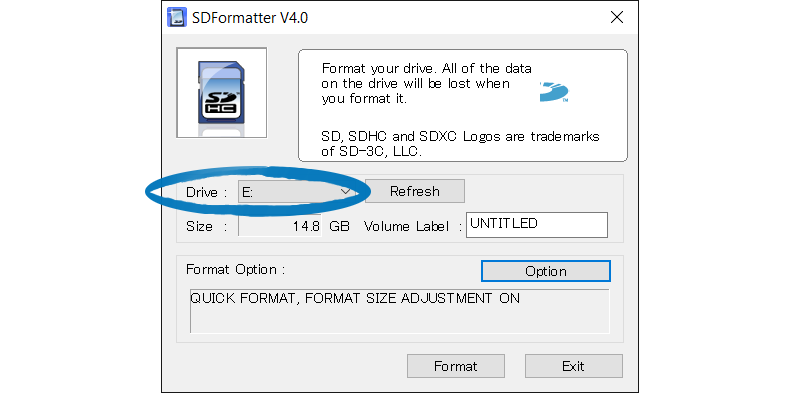
\includegraphics{images/SDFormatter.png}
	\caption{SDFormatter V4.0 Interface}
\end{figure}


\newpage
Before formatting the card, set the \textit{FORMAT SIZE ADJUSTMENT} to \menupath{ON} in the Option Settings as shown in \figref{fig:sdformatoption}. The \textit{FORMAT TYPE} can be left as \menupath{QUICK}. \\


\begin{marginfigure}
	\centering
	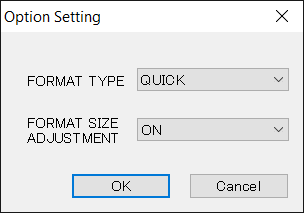
\includegraphics{images/SDFormatter_Option_Setting.png}
	\caption[Set Format Options in SDFormatter]{Set Format Options in SDFormatter}
	\label{fig:sdformatoption}
\end{marginfigure}


After setting the format options, select \menupath{Format} from the SDFormatter interface to start formatting the disk.


%\begin{figure}
%	\centering
%	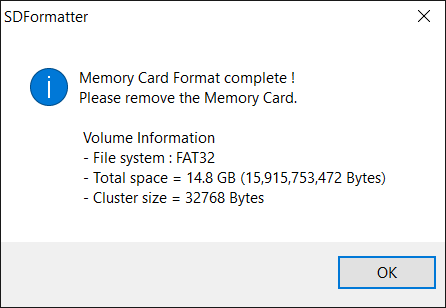
\includegraphics{images/SDFormatter_Complete.png}
%\end{figure}



%%%--------- Load the microSD Card Image ------------
\subsection{Load the microSD Card Image}

Before loading the Linux system on the microSD card, first download the system image. SD card images, as well as Linux system components and filesystems can be downloaded from \href{http://krtkl.com/downloads/}{krtkl}. The SD card image represents a 4GB SD card but can be loaded onto any size microSD card of 4GB or larger size. The compressed image is much smaller than 4GB as the system does not use nearly the full size of a 4GB card. After downloading, extract the system image to a convenient directory that will be accessed when writing the image to the card. \\

The Win32 Disk Imager utility is used to write the disk image to the freshly formatted microSD card. Download the utility from \href{http://sourceforge.net/projects/win32diskimager}{SourceForge} and install it on the Windows host. \\

\begin{figure}
	\centering
	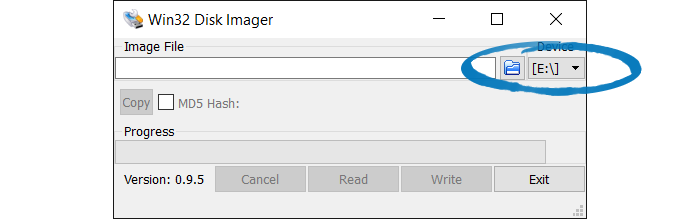
\includegraphics{images/Win32_Disk_Imager.png}
	\caption{Win32 Disk Imager Disk Letter Selection}
\end{figure}

After opening the Win32 Disk Imager, verify the drive letter matches that of the newly formatted card. By selecting the folder button next to the image file path, you will be able to navigate to and select the extracted system image file. After selecting the system image, select \menupath{Write} to begin writing the image to the microSD card, as shown in \figref{fig:win32diskimagewrite}. \\


\begin{figure}
	\centering
	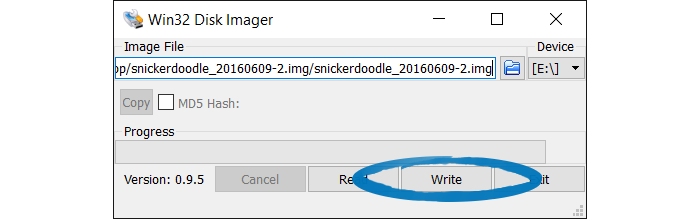
\includegraphics{images/Win32_Disk_Imager_Write_Image.png}
	\caption{Write Linux System Disk Image with Win32 Disk Imager}
	\label{fig:win32diskimagewrite}
\end{figure}


When the Win32 Disk Imager is finished writing the Linux system to the microSD card it can be ejected from the Windows host and loaded on Snickerdoodle. After mounting the microSD, Snickerdoodle can be powered on and booted from the microSD card. %For information on connecting to the Snickerdoodle Linux console, refer to \chapref{ch:usbvirtualcomport}. 

% -----------------------------------------------------
% 		Load microSD Card Using OS X
% -----------------------------------------------------
\section{Load microSD Card Using OS X}


OS X does not have native file system support for Linux filesystems. For this reason, the microSD card creation process parallels the process for Windows hosts. 


%%%--------- Format the microSD Card ----------
\subsection{Format the microSD Card}

The SD Association supports an SD card formatting utility for OS X machines. The utility can be downloaded from \href{https://www.sdcard.org/downloads/formatter_4}{SDCard.org}. After downloading and installing the SDFormatter, insert the microSD card and run the SDFormatter program. 





%%%--------- Load the microSD Card Image ------------
\subsection{Load the microSD Card Image}

Before attempting to copy the Linux system image to the microSD card, verify the disk location on the OS X host. \cmdstr{mount} can be used from a terminal to check the mount point of the newly formatted card. \lstref{lst:osxmountsd} shows the truncated output of the \cmdstr{mount} command, showing the disk label and \texttt{/dev} tree mount point. In this example, the disk labeled 'UNTITLED' is the first and only partition on \texttt{/dev/disk4} as it was created during the card formatting step (with its own file path \texttt{/dev/disk4s1}). 


\begin{lstlisting}[%
	style=text,
	caption=Verify microSD Card Location in OS X,
	label=lst:osxmountsd
]
$ mount
...
/dev/disk4s1 on /Volumes/UNTITLED (msdos, local, nodev, nosuid, noowners)
\end{lstlisting}


The formatted partition should be unmounted from the OS X host, before copying the Linux system image. Rather than using \cmdstr{umount}, the particularities of OS X require \texttt{diskutil unmount} be used to unmount the card's partition. 


\begin{lstlisting}[
	style=text,
	caption=Unmount microSD Card Partition in OS X,
	label=lst:osxunmountsd
]
$ diskutil unmount /dev/disk4s1
Volume UNTITLED on disk4s1 unmounted
\end{lstlisting}


\cautionnote{When loading the system image to the microSD card, do not include the partition in the output file name. In this example, \texttt{/dev/disk4s1} is the newly formatted FAT32 partition on \texttt{/dev/disk4} and so \texttt{/dev/disk4} is used as the output file for \cmdstr{dd}.}


\begin{lstlisting}[%
	style=text,
	caption=Load Linux System Image to microSD Card from OS X
]
$ sudo dd if=<image_path> of=/dev/disk4 bs=1m
\end{lstlisting}


After loading the image to the microSD card, the card can be ejected using \texttt{diskutil eject} and is ready to be loaded into Snickerdoodle.


\begin{lstlisting}	
$ sudo diskutil eject /dev/disk4
Disk /dev/disk4 ejected
\end{lstlisting}


After loading the microSD card, Snickerdoodle is ready to be powered on boot from the microSD card. %For information on connecting to the Snickerdoodle Linux console, refer to \chapref{ch:usbvirtualcomport}. 


% -----------------------------------------------------
% 		Create microSD Card Using Linux
% -----------------------------------------------------
\section{Create microSD Card Using Linux}

From a Linux environment, the microSD card can be created from the individual system components. This allows for greater flexibility in the configuration of the system and allows an opportunity to pre-load custom system components rather than replacing the components in the default configuration image.


%%%-------- Connecting and Locating the microSD Card ----------
\subsection{Connecting and Locating the microSD Card}

The \texttt{mount} command can be used to locate the SD card device, once it has been connected to the host computer. In the example below, an SD card has been connected on \texttt{/dev/sdb1} and mounted at \texttt{/media/user/UNTITLED}.


\begin{lstlisting}[style=text]
$ mount
/dev/sda1 on / type ext4 (rw,errors=remount-ro)
proc on /proc type proc (rw,noexec,nosuid,nodev)
sysfs on /sys type sysfs (rw,noexec,nosuid,nodev)
none on /sys/fs/cgroup type tmpfs (rw)
none on /sys/fs/fuse/connections type fusectl (rw)
none on /sys/kernel/debug type debugfs (rw)
...
(*@\bfseries\color{red}{/dev/sdb1}@*) on (*@\bfseries\color{red}{/media/user/UNTITLED}@*) type vfat (rw,nosuid,nodev,uid=1000,gid=1000,shortname=mixed,dmask=0077, utf8=1,showexec,flush,uhelper=udisks2)
\end{lstlisting}


%%%-------- Partitioning the microSD Card (fdisk) ---------
\subsection{Partitioning the microSD Card (\cmdstr{fdisk})}
Before partitioning the SD card, any partitions that have been mounted on the system must be unmounted. This can be done using the \texttt{umount} command.


\begin{lstlisting}
$ umount /dev/sdb1
\end{lstlisting}


Once the SD card has been located, we can partition it for the Linux system (\textit{BOOT} partition) and root filesystem (\textit{ROOTFS} partition) using \href{http://linux.die.net/man/8/fdisk}{\cmdstr{fdisk}}. Additional information on \cmdstr{fdisk} is available from the \href{http://tldp.org/HOWTO/Partition/fdisk_partitioning.html}{Linux Documentation Project}. \cmdstr{fdisk} must be run with root permissions (\texttt{sudo}) using the disk parent as the argument (do not use the parition number in the argument). 


\begin{lstlisting}[style=text]
$ fdisk /dev/sdb
\end{lstlisting}


\margincautionnote{Do NOT include any partition number (in the example case '1') when running \cmdstr{fdisk} on the SD card. '\texttt{/dev/sdb}' NOT '\texttt{/dev/sdb1}'}

From within the \texttt{fdisk} interface, we can view the parition table at any time using the 'p' command. In this example, an 8GB SD card with a single FAT32 partition is being used and will be re-partitioned for snickerdoodle.


\begin{lstlisting}[style=text]
Command (m for help): (*@\bfseries\color{red}{p}@*)

Disk /dev/sdb: 7969 MB, 7969177600 bytes
255 heads, 63 sectors/track, 968 cylinders, total 15564800 sectors
Units = sectors of 1 * 512 = 512 bytes
Sector size (logical/physical): 512 bytes / 512 bytes
I/O size (minimum/optimal): 512 bytes / 512 bytes
Disk identifier: 0x00000000

   Device Boot      Start         End      Blocks   Id  System
/dev/sdb1            8192    15564799     7778304    b  W95 FAT32
\end{lstlisting}


%%%-------- BOOT Partition -------
\subsection{BOOT Partition}
First, a partition must be allocated for the Linux system binaries and files. This includes \file{BOOT.bin} (FSBL, bitstream, U-Boot), \file{uEnv.txt}, \file{devicetree.dtb}, and the Linux kernel \file{uImage}. The partition size for these files is recommended to be 128MB in size which translates to an additional 262144, 512 byte sectors.


\clearpage
\begin{lstlisting}[style=text]
Command (m for help): (*@\bfseries\color{red}{d}@*)
Selected partition 1

Command (m for help): (*@\bfseries\color{red}{n}@*)
Partition type:
   p   primary (0 primary, 0 extended, 4 free)
   e   extended
Select (default p): (*@\bfseries\color{red}{p}@*)
Partition number (1-4, default 1): (*@\bfseries\color{red}{1}@*)
First sector (2048-15564799, default 2048): (*@\bfseries\color{red}{<RETURN>}@*)
Using default value 2048
Last sector, +sectors or +size{K,M,G} (2048-15564799, default 15564799): (*@\bfseries\color{red}{+262144}@*)
\end{lstlisting}



The default partition type for \cmdstr{fdisk} is \textbf{Linux} (type ID 83). The \textit{BOOT} partition needs to be formatted as \textbf{FAT32} (type ID 'C'). To do this, the 't' command is used:


\begin{lstlisting}[style=text]
Command (m for help): (*@\bfseries\color{red}{t}@*)
Partition number (1-4): (*@\bfseries\color{red}{1}@*)
Hex code (type L to list codes): (*@\bfseries\color{red}{c}@*)
Changed system type of partition 1 to c (W95 FAT32 (LBA))
\end{lstlisting}


%%%-------- ROOTFS Partition --------
\subsection{ROOTFS Partition}
Second, a partition for the root filesystem must be created. This partition will be formatted as a \textbf{Linux} type using type ID 83. This is the default partition type.


\begin{lstlisting}[style=text]
Command (m for help): (*@\bfseries\color{red}{n}@*)
Partition type:
   p   primary (1 primary, 0 extended, 3 free)
   e   extended
Select (default p): (*@\bfseries\color{red}{p}@*)
Partition number (1-4, default 2): (*@\bfseries\color{red}{<RETURN>}@*)
Using default value 2
First sector (264193-15564799, default 264193): (*@\bfseries\color{red}{<RETURN>}@*)
Using default value 264193
Last sector, +sectors or +size{K,M,G} (264193-15564799, default 15564799): (*@\bfseries\color{red}{<RETURN>}@*)
Using default value 15564799
\end{lstlisting}

\margininfonote{Always check the partition table before attempting to write it to the disk, using the 'p' command.}


Before writing the partition table, you should verify the partition layout by printing it with the 'p' command. In this example, an 8GB SD card has been partitioned with a 128MB FAT32 \textit{BOOT} partition and the rest allocated for a Linux \textit{ROOTFS} partition.


\begin{lstlisting}[style=text]
Command (m for help): (*@\bfseries\color{red}{p}@*)

Disk /dev/sdb: 7969 MB, 7969177600 bytes
255 heads, 63 sectors/track, 968 cylinders, total 15564800 sectors
Units = sectors of 1 * 512 = 512 bytes
Sector size (logical/physical): 512 bytes / 512 bytes
I/O size (minimum/optimal): 512 bytes / 512 bytes
Disk identifier: 0x00000000

   Device Boot      Start         End      Blocks   Id  System
/dev/sdb1            2048      264192      131072+   c  W95 FAT32 (LBA)
/dev/sdb2          264193    15564799     7650303+  83  Linux
\end{lstlisting}


Once the partition table has been verified, the 'w' command can be used to write the table to the disk:


\begin{lstlisting}[style=text]
Command (m for help): (*@\bfseries\color{red}{w}@*)
The partition table has been altered!

Calling ioctl() to re-read partition table.
Syncing disks.
\end{lstlisting}


%%%-------- Formatting Partitions (mkfs/mke2fs) --------
\subsection{Formatting Partitions (\cmdstr{mkfs}/\cmdstr{mke2fs})}
With a partitioned SD card, the partitions need to be formatted with the necessary filesystem type. For the \textit{BOOT} partition, the filesystem type is \textbf{VFAT}. Formatting the \textit{BOOT} partition can be done using the \texttt{mkfs.vfat}\sidenote{Additional information on \texttt{mkfs/mke2fs} and its front end tools can be found at: \url{http://www.tldp.org/HOWTO/Partition/formatting.html}}. To format a FAT32 filesystem on \texttt{/dev/sdb1} with a 'BOOT' disk label, the following command can be used:


\begin{lstlisting}
$ mkfs.vfat -n BOOT /dev/sdb1
\end{lstlisting}


The format for the \textit{ROOTFS} partition can be done with \texttt{mke2fs} which will format a Linux partition with an ext2/ext3/ext4 filesystem. To format an ext4 filesystem on \texttt{/dev/sdb2} with a block size of 1k (1024) and a 'ROOTFS' disk label, the following command can be used:

\margincautionnote{When formatting disk partitions, make sure the disk partitions are NOT mounted.}


\begin{lstlisting}
$ mke2fs -b 1024 -t ext4 -L ROOTFS /dev/sdb2
\end{lstlisting}


If the formatting is successful, the following output with be written to the console (writing superblocks and filesystem accounting information can take some time depending on the size and speed of the SD card):


\begin{lstlisting}[style=text]
mke2fs 1.42.9 (4-Feb-2014)
Filesystem label=ROOTFS
OS type: Linux
Block size=4096 (log=0)
Fragment size=4096 (log=0)
Stride=0 blocks, Stripe width=0 blocks
478208 inodes, 7650300 blocks
382515 blocks (5.00%) reserved for the super user
First data block=1
Maximum filesystem blocks=74973184
934 block groups
8192 blocks per group, 8192 fragments per group
512 inodes per group
Superblock backups stored on blocks: 
	8193, 24577, 40961, 57345, 73729, 204801, 221185, 401409, 663553, 
	1024001, 1990657, 2809857, 5120001, 5971969

Allocating group tables: done                            
Writing inode tables: done                            
Creating journal (32768 blocks): done
Writing superblocks and filesystem accounting information: done   
\end{lstlisting}


After the partitions have been properly formatted, the SD card must be ejected and re-connected before moving the Linux boot components and root filesystem contents to the disk.


\begin{lstlisting}
$ eject /dev/sdb
\end{lstlisting}


%%%-------- BOOT Partition Components ---------
\subsection{BOOT Partition Components}

The latest \textit{BOOT} partition Linux components for Snickerdoodle and Snickerdoodle Black can be downloaded using \texttt{git}.


\begin{fullwidth}
\begin{lstlisting}[style=text]
$ git clone https://github.com/krtkl/snickerdoodle-linux-prebuilt.git
\end{lstlisting}
\end{fullwidth}


Alternatively, the sources can be downloaded directly from a web browser from the \href{https://github.com/krtkl/snickerdoodle-linux-prebuilt}{krtkl GitHub page} as a \texttt{.ZIP} file.

%\begin{figure}[h!]
%\centering
%	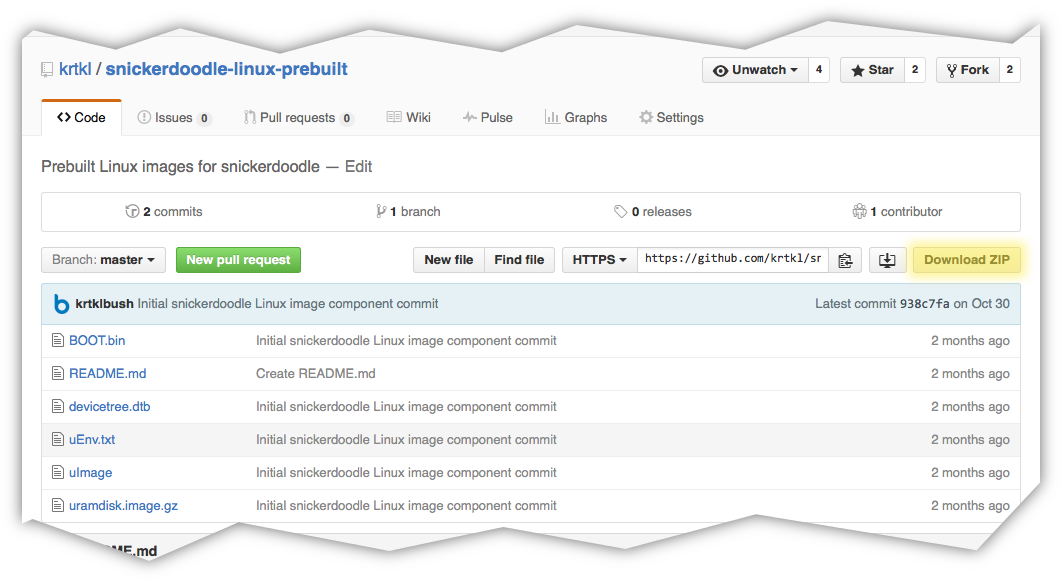
\includegraphics{images/github-prebuilt.png}
%	\caption{Download prebuilt Linux components from GitHub}
%	\label{fig:githubprebuilt}
%\end{figure}


%%%-------- Copy Files to SD Card --------
\subsection{Copy Files to SD Card}
After downloading the SD card components


The \textit{BOOT} components can be installed onto the SD card using the \texttt{cp} command, starting with \texttt{BOOT.bin}. In this example, the files are copied to the \textit{BOOT} partition that has been mounted at \texttt{/media/user/BOOT}. As stated above, the \texttt{mount} command can be used to \hyperref[sub:locatesd]{locate the mount point of the SD card partitions}.


\begin{lstlisting}
$ cp BOOT.bin /media/user/BOOT
$ cp uEnv.txt /media/user/BOOT
$ cp devicetree.dtb /media/user/BOOT
$ cp uImage /media/user/BOOT
\end{lstlisting}


After copying the \textit{BOOT} components, the \texttt{sync} command should be used to make sure the system buffers have been flushed and the process of writing the files to the SD card is complete.


\begin{lstlisting}
$ sync
\end{lstlisting}


%%%-------- ROOTFS Sources --------
\subsection{ROOTFS Sources}

The root filesystem can be extracted directly into the \textit{ROOTFS} partition using the '-C' argument when extracting the archive contents. An Ubuntu 14.04 filesystem can be downloaded from \url{http://krtkl.com/downloads/}. In this example, the \textit{ROOTFS} partition is mounted at \texttt{/media/user/ROOTFS}, which should be checked before attempting to extract the root filesystem. The root filesystem contains a lot of large packages (ROS, python, etc.) and may take several minutes to complete the process of writing to the SD card.


\begin{fullwidth}
\begin{lstlisting}
$ tar -C /media/user/ROOTFS -xvzf snickerdoodle-ubuntu-14.04.tar.gz
\end{lstlisting}
\end{fullwidth}


After extracting the root filesystem to the SD card, use the \texttt{sync} command to flush the system buffers and ensure the write process is complete. Additionally, making sure to unmount the SD card partitions before ejecting will make certain that any lingering write processes have completed before the SD card is removed.


\begin{lstlisting}
$ sync
$ umount /dev/sdb1
$ umount /dev/sdb2
$ eject /dev/sdb
\end{lstlisting}





